\section{Experimental evaluation}
\label{sec:results}
We conduct experiments to evaluate the performance of \tmatam on 
real world data. We present our results as follows. 
Section~\ref{subsec:summary} highlights the key insights drawn 
from our experiments. Section~\ref{subsec:setup} describes the 
experimental setup including the datasets and test-bench. In 
Section~\ref{subsec:perf1}, we compare \tmatam against previous 
state-of-the-art approaches. That is followed by a detailed study of
the behavior of \tmatam in Section~\ref{subsec:perf2}. Finally, 
a qualitative analysis of \tmatam's results in Section~\ref{subsec:qualitative}.

\begin{figure}[t!]
\centering
\frame{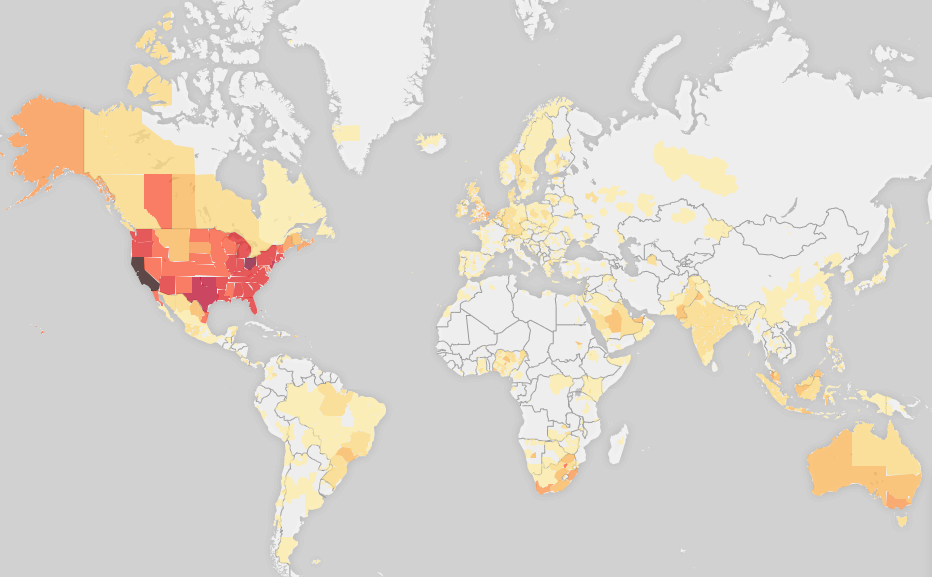
\includegraphics[width=0.45\textwidth]{heatmap/heatmap}}
\caption{Heatmap over collected health tweets. A major fraction
of the tweets originate from various states in the US.}
\label{fig:data:heatmap}
\end{figure}

\subsection{Summary of results}
\label{subsec:summary}
By modeling transitions in the same \change, TM–ATAM
consistently outperforms \tmlda in predicting 
health topics in all social-media active regions.

We analyze the performance of \tmatam by changing spatio-temporal parameters.
In particular, we find that prediction accuracy for health topics is higher when operating \tmatam on finer spatial granularity and shorter time periods.

Further, we go on to discover interesting region-specific intra and inter-\change health-related transitions. 
While studying these transitions, we find that \changes are continuous time periods for which people in the same region tweet about similar health issues. When those \changes end, we found that ailments discussed in Twitter transition into other ailment topics.
These results show that it is more logical to predict future ailments concerning people within the same \change of a
region than on any random health tweets.

By outperforming \tmlda in predicting future health topics, we show that it is essential 
to use a dedicated method that separates health-related topics from other topics. 

\begin{table}
\centering
\caption{Dataset Statistics}
\label{tab:data:stats}
\begin{tabular}{|c||c|}
\hline
collection period (days) & 235\\
\hline
\#tweets & {1,360,705,803}\\
\hline
\#tweets (health-related) & 698,212\\
\hline
\#tweets (health-related+geolocated) & 569,408\\
\hline
\end{tabular}
\end{table}
\subsection{Setup}
\label{subsec:setup}
\subsubsection{Data}

We employ Twitter's Streaming API to collect tweets. We use the \emph{Decahose Stream}\footnote{\url{https://dev.Twitter.com/streaming/overview}} which gives a $10\%$ random sample of the total tweets generated 
each day. We collect tweets for the period $2014$-Oct-$8$ to $2015$-May-$31$.
The collected tweets were subjected to two preprocessing steps described next.

{\bf Filtering health-related tweets:} Since our interest lies 
in public health discourse on social media, we filter the tweets 
returned by the \emph{Decahose Stream} to obtain \emph{health-related} 
tweets. We say that a tweet is health-related if it has a health 
keyword and passes our classification criteria.
The process is automated with the help of an SVM classifier
 ~\cite{DBLP:journals/ml/CortesV95}
with linear kernel and uni-gram, bi-gram and tri-gram word 
features. To this end, a modest-sized sample of the original 
corpus was annotated through crowdsourcing efforts where annotators 
were asked to label $5128$ tweets. The precision and recall of the 
employed classifier are $0.85$ and $0.44$. Table~\ref{tab:data:stats} 
shows that out of the 1.36B tweets we collected, 689K were health-related. 

{\bf Geolocation:} The ability to operate seamlessly at varying 
geographic resolutions mandates that the exact location of each 
tweet be known to \tmatam. Twitter affords its users the option 
to share their geolocation. It has been shown that a very small 
number of Twitter users choose to share their location. While 
this artefact results in significant reduction in the number of 
tweets, in absolute terms, we retain more than half a million 
tweets ($569K$ as indicated in Table~\ref{tab:data:stats}). 
% \comment{
% 	Note that recently, the problem of automated geotagging of tweets 
% 	has drawn attention of the research community and several solutions 
% 	have been proposed. In this work, we refrain from using any such 
% 	strategy and use a simple filtering scheme to retain tweets that 
% 	could be geolocated. 
% }
In Figure~\ref{fig:data:heatmap}, we present a heatmap that shows 
the geographic spread of these tweets. The darker the color, 
the higher the number of tweets. The top-10 regions (at spatial 
granularity \emph{state}) with the highest number of health tweets 
lie exclusively in the US.

\subsubsection{Test-Bench}
We run our experiments on a {32 core Intel Xeon @ 2.6Ghz CPU 
(with 20MB cache per core)} system with {128 Gig} RAM running 
{Debian GNU/Linux 7.9 (wheezy)} operating system.
All subsequently discussed components were implemented in 
Java {1.8.0\_60}.

\subsection{\tmatam vs \tmlda}
\label{subsec:perf1}
% \comment{
% 	\subsubsec{\change Detection at geographic granularity state and temporal granularity month}
% 	\label{subsubsec:season2}
% 	We first observe that it is unlikely for a county to exhibit health 
% 	patterns independent and different from its neighboring counties. 
% 	We hence decide to operate at the state level and obtain $1938$ states, 
% 	but not all of them are active tweeters on health. We choose to 
% 	filter only those \textit{active states} with at least one tweet 
% 	per week for the entire time period. We get 66 such active states. 
% 	We run ATAM~\cite{atam2} on health tweets of each state and convert its
% 	output into $monthly$ distributions as described in Algorithm~\ref{alg:tmatam}. 
% 	We do not choose to instantiate with $week$ as weekly distributions 
% 	were found to be too sparse. Our distribution vectors consist of 
% 	both ailment topics and general-purpose topics. We compute the 
% 	Bhattacharya Distance between topic distributions of
% 	consecutive months. The month-pair with the highest distance is 
% 	termed as \textit{change point} and the time period
% 	before and after the \textit{change point} are termed as $\changes$ 
% 	as defined in Section~\ref{sec:background}. Figure~\ref{fig:ailmentsEvolve}
% 	shows December to January as the \textit{change point}s for Kuala Lumpur. 
% }

\subsubsection{Perplexity Measure}
\begin{table}[t!]
\centering
\caption{Default Parameters}
\label{tab:parameters}
\begin{tabular}{|c|c|c|}
\hline
{\bf Term} &{\bf Description} & {\bf Value}\\
\hline
$\mf G$ &Geographic granularity &\emph{states}\\
\hline
$\mf T$ &Temporal granularity &\emph{months}\\
\hline
$m$ &Distance measure&\emph{Bhattacharya}\\
\hline
\end{tabular}
\end{table}
We use \emph{perplexity}, an empirical measure often used in NLP.
\footnote{\url{https://en.wikipedia.org/wiki/Perplexity}}
Perplexity of a language model measures how accurately the model can 
explain previously unseen data/documents. Given a language model
$l$ and a document $d$, perplexity is defined as below.
\begin{equation}
        \label{eq:perplexity}
	Perplexity(l) = 2^{-\sum_{w_i\in d} \log p_l(w_i)}
\end{equation}
This formula of perplexity for a document $d$ can be converted to a formula of perplexity for a set of documents $D_g^t$ as follows:
\begin{equation}
        \label{eq:perplexityGeoTemp}
	Perplexity\_{D_g^t}(l) = 2^{-\sum_{w_i\in d} \log \frac{\sum_{d\in D_g^t}p_l(w_i)}{|D_g^t|}}
\end{equation}
Formula \ref{eq:perplexityGeoTemp} denotes the perplexity of language model $l$ on a document-set at geo-granularity $g$ and temporal granularity $t$. 
Higher probability of words that occur in unseen documents results in lower perplexity and is hence better.
Here, $p_l(w_i)$ is the probability of occurrence of word $w_i$ as 
estimated by the language model $l$ in the document set. Previously unseen words can result in infinite perplexity. We use add-one smoothing to overcome this fact \footnote{\url{https://en.wikipedia.org/wiki/Additive_smoothing}}.
We compute perplexity of \tmatam and then compare perplexity of \tmatam with that of \tmlda on the same test document set  $D_g^t$ as explained in the next section. Both \tmatam and \tmlda are treated as  language models
as both give out probability of each word for any document-set $D_g^t$.
% \comment{
% 	\begin{figure}[t!]
% 	\centering
% 	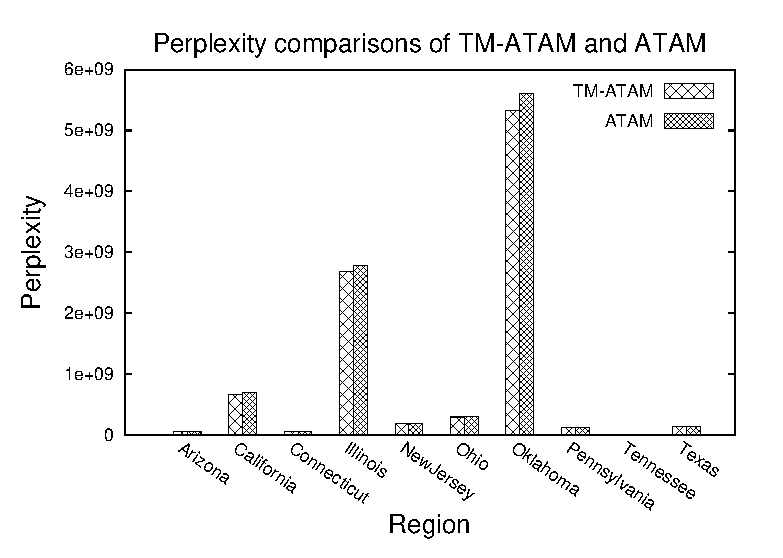
\epsfig{file=gnuplot/perplexity/perplexityAtamUS,width=0.45\textwidth}
% 	\caption{\tmatam and \atam prediction accuracies for top-10  active US states.}
% 	\label{fig:perplexityAtam}
% 	\end{figure}
% 	\begin{figure}[t!]
% 	\centering
% 	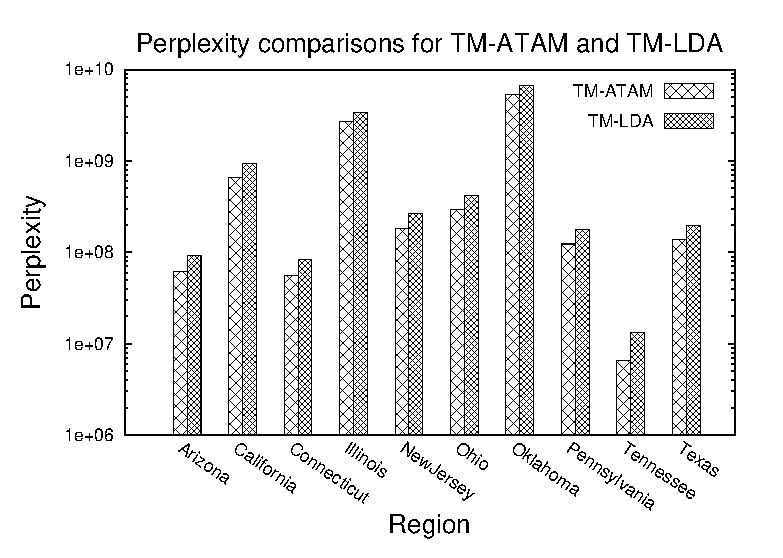
\epsfig{file=gnuplot/perplexity/perplexityUS,width=0.45\textwidth}
% 	\caption{\tmatam and \tmlda prediction accuracies for top-10  active US states.}
% 	\label{fig:perplexity1}
% 	\end{figure}
% 	\begin{figure}[t!]
% 	\centering
% 	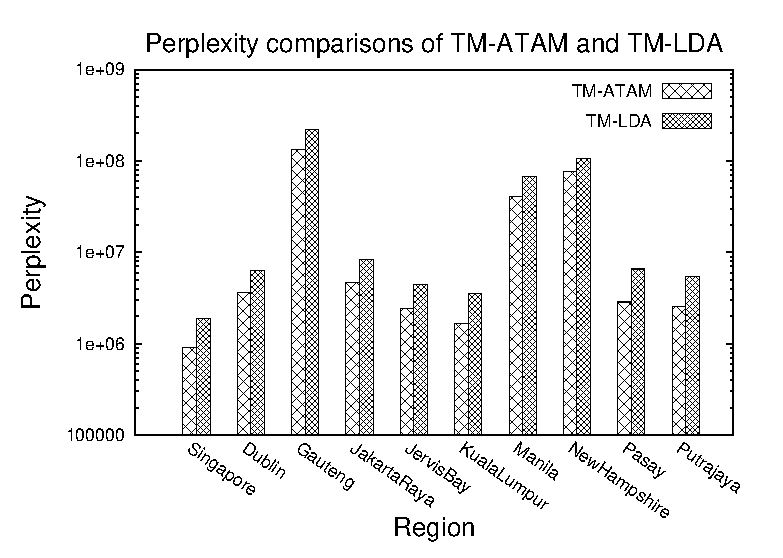
\epsfig{file=gnuplot/perplexity/perplexityNonUS,width=0.47\textwidth}
% 	\caption{\tmatam and \tmlda prediction accuracies for top-10 active non-US states.}
% 	\label{fig:perplexity2}
% 	\end{figure}
% }

\begin{figure*}[t!]
\centering
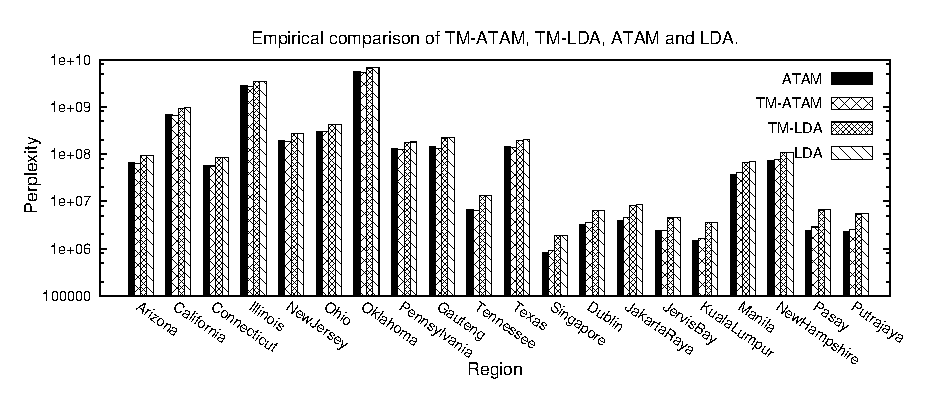
\epsfig{file=gnuplot/perplexity/perplexity,width=0.95\textwidth}
\caption{Perplexity comparison of \tmatam,\tmlda and \atam for top 20 social media active regions.}
\label{fig:perplexity}
\end{figure*}

\subsubsection{Comparing \tmatam with \tmlda and \atam}
We present results on the comparison of prediction accuracy of \tmatam
against \tmlda. We first divide the postings of each region into two 
\changes as inferred by $t_{c}$. We then divide each \change into train and test set as follows.
$Pre$-\change is divided into  train $([t_1\ ,t_{c-3}])$ and test $([t_{c-2},t_{c-1}])$ set. $post$-\change is divided into
train $([t_{c+1},t_{|\mf T|-2}])$ and a test $([t_{|\mf T|-1},t_{|\mf T|}])$ set. For example, if $t_c$ for a region is between January to February, then train set and test set of $pre$-\change are tweet posts of the months in the set [October,December] and [January,February] respectively. Train and test set of $post$-\change are tweet posts of months in the set [March,April] and  [May,June] respectively.
 We obtain 69 \changes for 66 regions. ATAM is \textit{re-run} over train set of each \change. It should be noted that though computing \textit{change point $t_c$} required access to full dataset, perplexity calculations are done within each \change and clear distinction is made between train and test set while computing it.  We then model a transition matrix 
$M_{tmatam}$ on the training data of each \change as described in Section~\ref{subsec:tmalg}. 
For each tweet $p$ of the first month in the test set $(t_{c-2}$ for the $pre$ \change and $t_{|\mf T|-1}$ for the $post$ \change), 
we compute the probability of "health topic" $z$ using the following formulas: \\
\begin{equation}
\label{eq:probabilitytopicgiventimepre}
P(z|t_{c-2}) = \frac{\sum_{p\ over\ the\ t_{c-2}}P(z|p\ for\ t_{c-2} )}
    {number\ of\ tweets\ for\ t_{c-2}}
\end{equation}
\begin{equation}
\label{eq:probabilitytopicgiventimepost}
P(z|t_{|\mf T|-1}) = \frac{\sum_{p\ over\ the\ t_{|\mf T|-1}}P(z|p\ for\ t_{|\mf T|-1} )}
    {number\ of\ tweets\ for\ t_{|\mf T|-1}}
\end{equation}
 Here $P(z|p)$ is computed simply by ($w$ is the word of tweet $p$): \\
\begin{equation}
\label{eq:probabilitytopicgiventweet}
 P(z|p)=\sum_{w}P(z|w)P(w|p) = \sum_{w}\frac{n(z,w)}{n(w)}P(w|p)
\end{equation}
Here, values for $n(z,w)$,$n(w)$ are taken from ATAM run on the training months. If we encounter an unseen word, we use add-one smoothing to avoid $P(w|p)$  to shoot to infinity and hence perplexity to shoot to infinity. P(z|w) is simply the number of times word $w$
occurs in the tweet $p$ divided by the total number of words in the tweet $p$.
We then predict the future probability of each topic in the 
second month of the test data ($P(z|t_{c-1})$ for $pre$ \change and $P(z|t_{|\mf T|})$ for the $post$ \change) using the corresponding transition matrix $M_{tmatam}$. The perplexity of \tmatam can now be computed against the words of the tweets of second test month ($t_{c-1}$ and $t_{|\mf T|}$)  using the formula~\ref{eq:perplexityGeoTemp}. This gives 69 values of perplexity, 
one for each \change of each region. We compare our results with following competitors:
\begin{itemize}
\item \atam: In order to assert the fact that health topics transit from one to another, we compare performance of \tmatam with \atam by computing perplexity of \atam on words of first month of test set and not predicting any topic distribution using transition matrix. For each tweet p of the first month in the test set ($t_{c-2}$ for the $pre$ \change and $t_{|\mf T|-1}$ for the $post$ \change), we compute the probability of "health topic" z using the formulas \ref{eq:probabilitytopicgiventimepre},\ref{eq:probabilitytopicgiventimepost},\ref{eq:probabilitytopicgiventweet}. It should be noted that in this case \textit{we do not model a transition matrix to predict probability of topics for second month of test set}. Hence, this denotes model where health topics stay \textit{static}. We can then compute perplexity of \atam against words of actual tweets of the first months of test month $(t_{c-2}$ and $t_{|\mf T|-1}$).  As shown in figure \ref{fig:perplexity}, \tmatam beats \atam in all US active regions. In Non-US active regions, the performance of \tmatam gets affected due to no substantial change in health topics with time.
\item Predicted \tmlda: Each region can be viewed as a 
\texttt{virtual user} and the transition matrix $M_{tmlda}$ of \tmlda is trained
by solving least squares problem in the following manner. We merge 
the training data of each \change in each region and train a transition
matrix of \tmlda. So, training data for \tmlda is the same as that of \tmatam: $([t_1\ ,t_{c-3}])$ for the $pre$ \change and $([t_{c+1},t_{|\mf T|-2}])$ for the $post$ \change.
% \comment{
% 	\begin{figure}[b!]
% 	\centering
% 	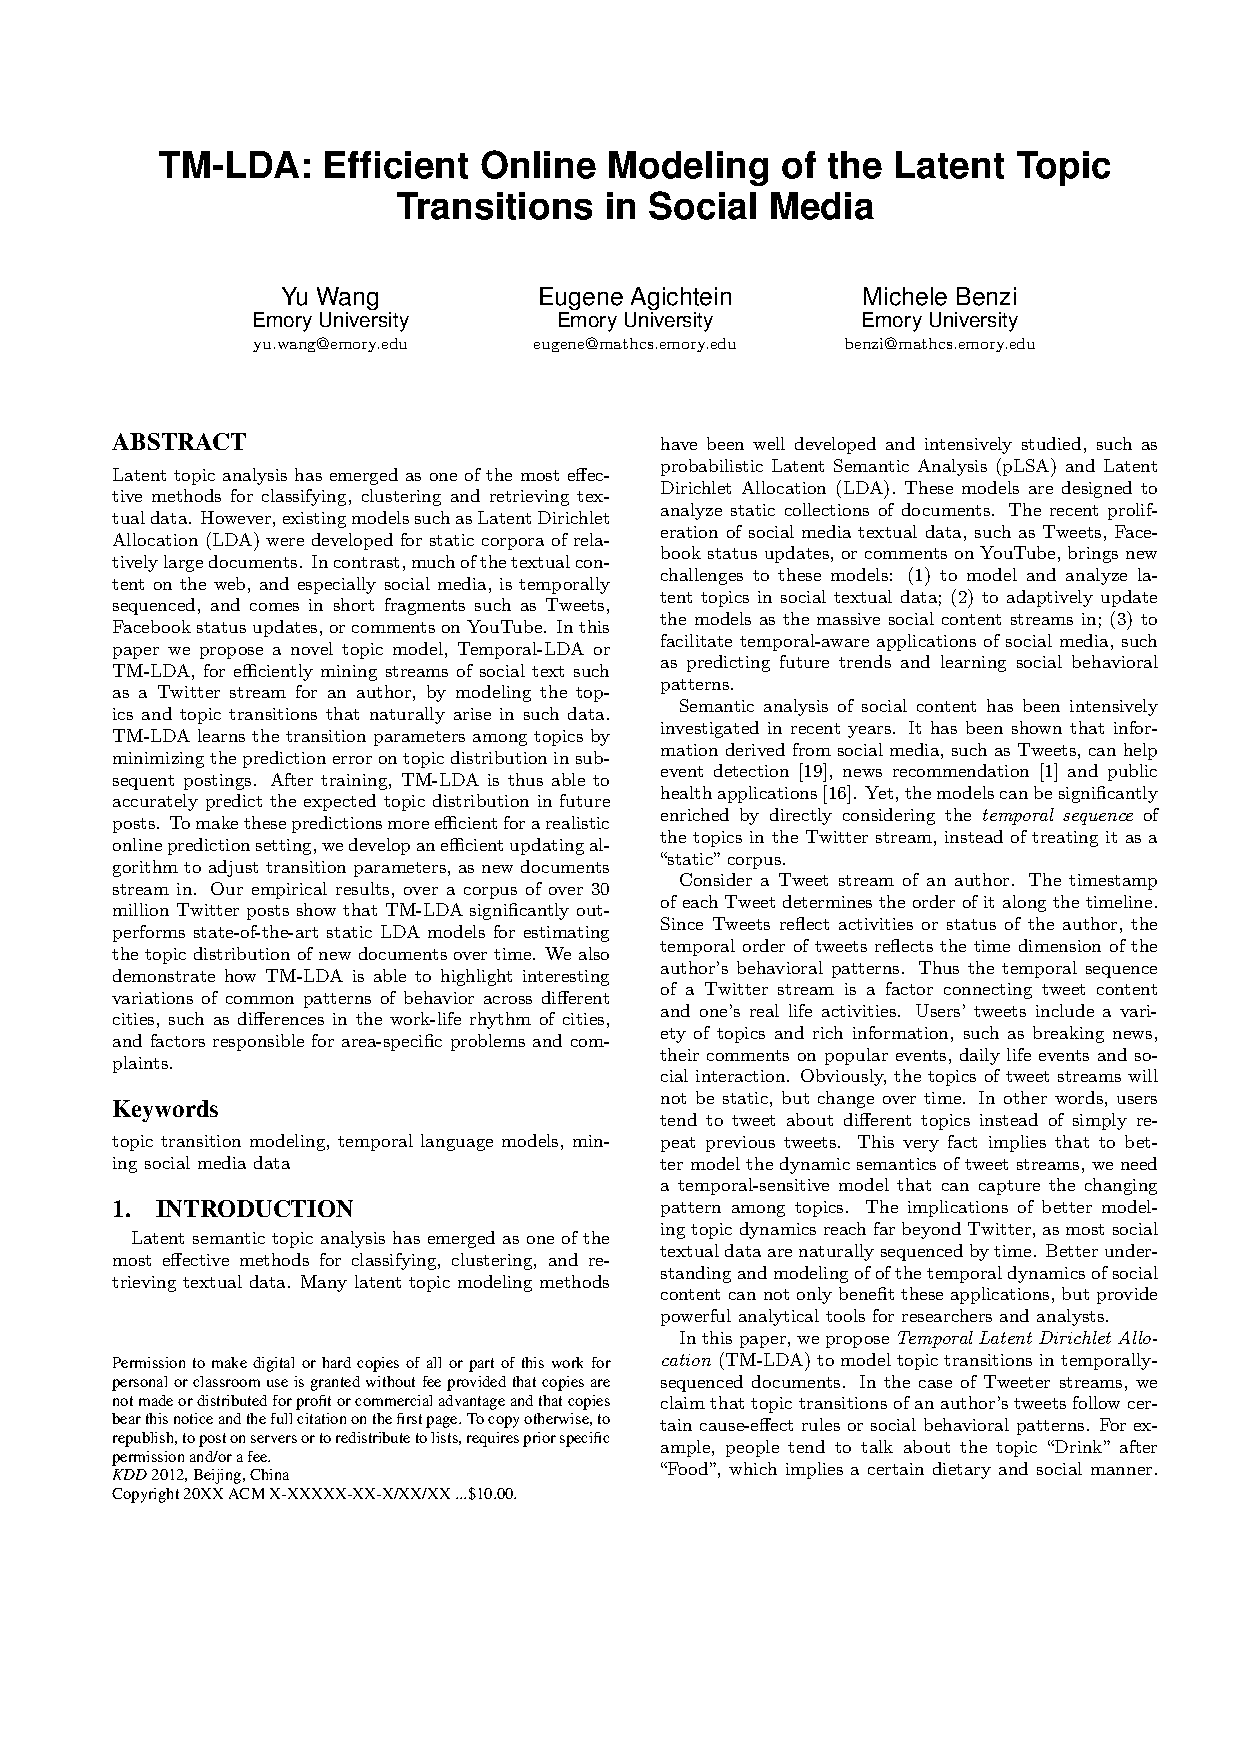
\includegraphics[width=0.45\textwidth]{tikz/tmlda.pdf}
% 	\caption{TM-LDA Model}
% 	\label{fig:tmlda}
% 	\end{figure}
% }
For each tweet $p$ of the first month of the test months $(t_{c-2}$ and $t_{|\mf T|-1}$), we compute the 
probability $P(z|t_{c-2})$ and $P(z|t_{|\mf T|-1})$ using LDA trained on merged training data (Formulas \ref{eq:probabilitytopicgiventimepre},\ref{eq:probabilitytopicgiventimepost},\ref{eq:probabilitytopicgiventweet}). We 
then predict the future probability of each topic in following month ($t_{c-1}$ and $t_{|\mf T|}$)
using corresponding $M_{tmlda}$. We can then compute the perplexity of \tmlda 
against words of actual tweets of the test months ($t_{c-1}$ and $t_{|\mf T|}$) using formula \ref{eq:perplexityGeoTemp} . 
\end{itemize}
$p_l(w_i)$, probability of word, for any document set is calculated as follows:
\begin{equation}
\label{eq:probabilityword}
p_l(w_i)=\sum_{z}P(w|z)P(z) = \sum_{z}\frac{n(z,w)}{n(z)}P(z)
\end{equation}
Here $P(z)$ is the probability of topic, which is computed by  multiplying corresponding transition matrix ($M_{tmatam}$ or $M_{tmlda}$) by the matrix formed during the training phase (\tmatam or \tmlda). Having computed P(w), we can compute perplexity using the formula \ref{eq:perplexityGeoTemp}. We take average over both \changes ($pre$ and $post$) and get a perplexity value for each region. 
Figures~\ref{fig:perplexity} and~\ref{fig:perplexity} show that \tmatam
consistently beats \tmlda in predicting
future health topics on the test month by computing lower perplexity on the words of the tweets of the test month in all social media active states.
\subsection{\tmatam: Effect of parameters}
\label{subsec:perf2}
\subsubsection{Geographic Granularity}
\begin{figure}[b!]
\centering
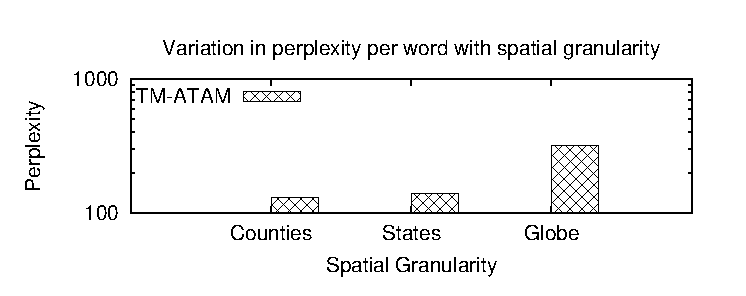
\epsfig{file=gnuplot/perplexity/perplexityGeographic,width=0.42\textwidth}
\caption{Variation in performance of \tmatam with geographic granularity over regions. "States" and "Counties" correspond to first and second level administrative divisions.}
\label{fig:perplexitySpatial}
\end{figure}
We examine two different choices for the geographic 
granularity i.e. \emph{states} and \emph{counties} which correspond to
first and second level administrative divisions. \footnote{\url{https://en.wikipedia.org/wiki/Table_of_administrative_divisions_by_country}}
While \tmatam can be instantiated at varying granularities of space, 
learning accurate ailment distributions requires a certain minimum number 
of tweets.  Selecting larger 
than optimal sized regions would introduce errors 
into the prediction algorithm. Choice of geographic granularity is non-trivial.
Predicted perplexity in counties is lower, hence better, than perplexity at the level of states as shown in Figure~\ref{fig:perplexitySpatial}.
We attribute this result to the fact that tweets from smaller regions show less diversity in topics.
\subsubsection{Temporal Granularity}
\begin{figure}[t!]
\centering
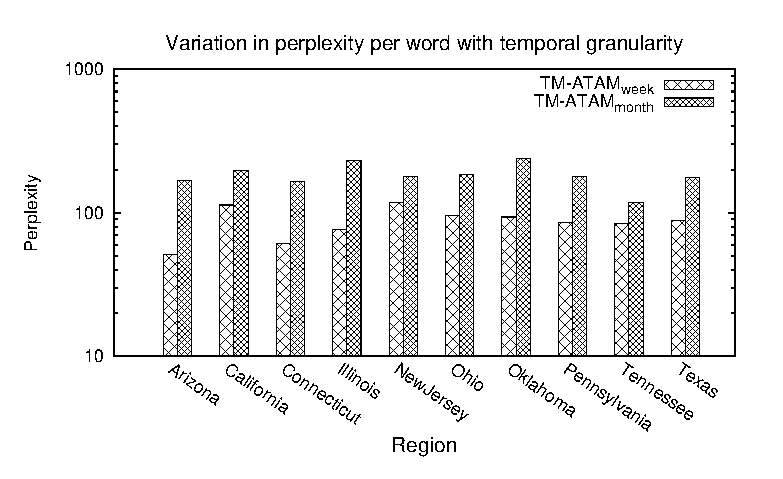
\epsfig{file=gnuplot/perplexity/perplexityTemporalUS,width=0.45\textwidth}
\caption{Variation in perplexity achieved by \tmatam at different 
temporal granularities. Results for top-10 social media active regions.}
\label{fig:perplexityTemporalUS}
\end{figure}
\begin{figure}[b!]
\centering
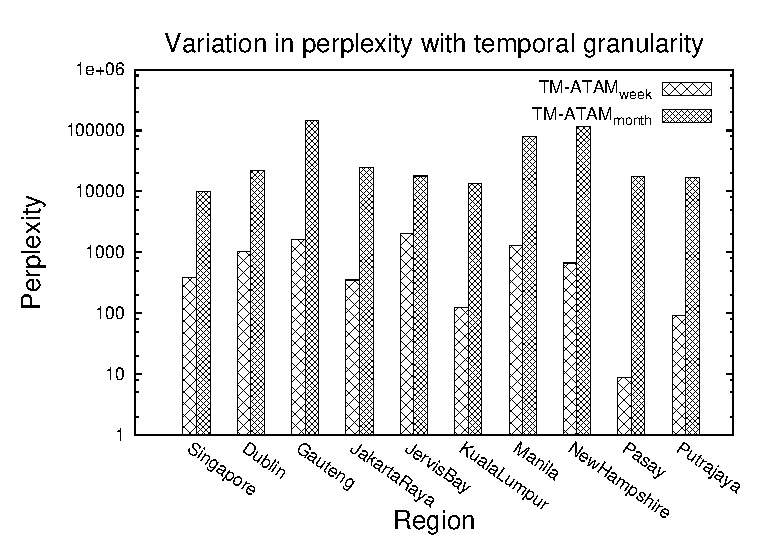
\epsfig{file=gnuplot/perplexity/perplexityTemporalNonUS,width=0.45\textwidth}
\caption{Variation in perplexity achieved by \tmatam at different 
temporal granularities. Results for top-10 non-US active regions.}
\label{fig:perplexityTemporalNonUS}
\end{figure}
We examine two different temporal granularities, \emph{months} 
and \emph{weeks}. Analogous to geographic granularity, choice of temporal 
granularity should not be too fine or too coarse. We show performance 
of \tmatam on time granularities in Figures~\ref{fig:perplexityTemporalUS} 
and \ref{fig:perplexityTemporalNonUS}. 
This is also attributed to the fact that prediction of health topics in smaller temporal granularity is more accurate as health topics do not transform by a substantial amount in shorter periods.
\subsubsection{Distance Measures}
The obtained \change-boundary depends on the choice of distance measure $m$.
We conduct experiments with two different measures, namely, Bhattacharya
Distance and Cosine Similarity. We convert the latter to a distance
measure $d=\sqrt{2-2\times cos}$ where $cos$ is the cosine similarity.
For each measure, we compute perplexity over \emph{pre} and \emph{post} 
time intervals. Results are shown in Figures~\ref{fig:perplexityMeasureUS} 
and \ref{fig:perplexityMeasureNonUS}. On an average over regions, 
Bhattacharya Distance outperforms Cosine Similarity. We observed that number of 
tweets at a given time granularity $t$ may affect the performance of Cosine Similarity. This may
happen even after normalizing the topic vectors into unit-length as some of the topics may not even get instantiated.
\begin{figure}[t!]
\centering
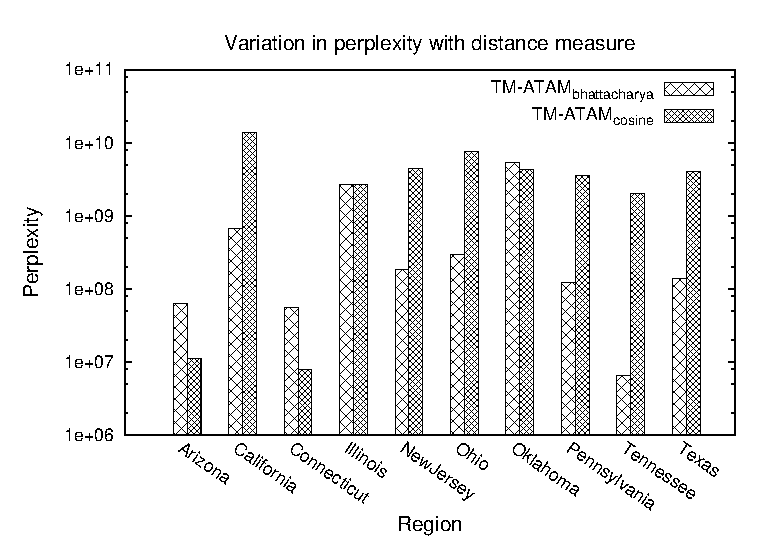
\epsfig{file=gnuplot/perplexity/perplexityMeasureUS.eps,width=0.45\textwidth}
\caption{Variation in perplexity achieved by \tmatam with different 
distance measures. Results computed over top-10 active U.S. regions.}
\label{fig:perplexityMeasureUS}
\end{figure}
\begin{figure}[t!]
\centering
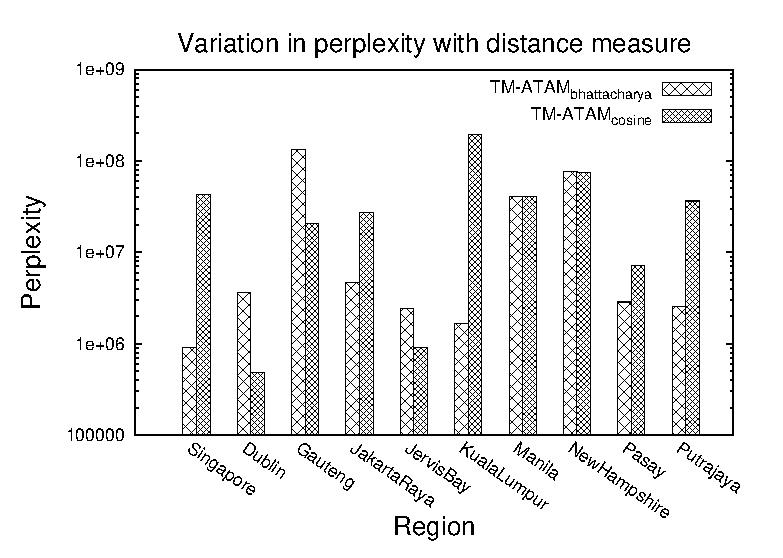
\epsfig{file=gnuplot/perplexity/perplexityMeasureNonUS.eps,width=0.45\textwidth}
\caption{Variation in perplexity achieved by
TM–ATAM with different distance measures. Results
computed over top-10 non-US active regions.}
\label{fig:perplexityMeasureNonUS}
\end{figure}
\subsection{Qualitative Analysis of \tmatam}
\label{subsec:qualitative}
\subsubsection{\changes}
\label{subsubsec:season}
The central idea in TM–ATAM is to identify \changes, i.e.,
time intervals that exhibit homogeneous ailment distributions, as well
as transitions between them.
A natural question that emerges is {\em how and why} ailments
differ across \change boundaries. In Figures 13 and 14
we show the sharpest change point, representing the strongest
transition, for the top-10 US and
non-US regions respectively. Those points can be explained with weather
changes in those regions. For example, Texas can be explained with a
drop in temperature while Jervis Bay can be explained by an increase in
rainfall. Dublin sees its lowest temperature in the November period.
Singapore and Manila have very similar weather conditions and exhibit
the same change point. A deeper look at these transitions would provide
more insights.
\begin{figure}[b!]
\centering
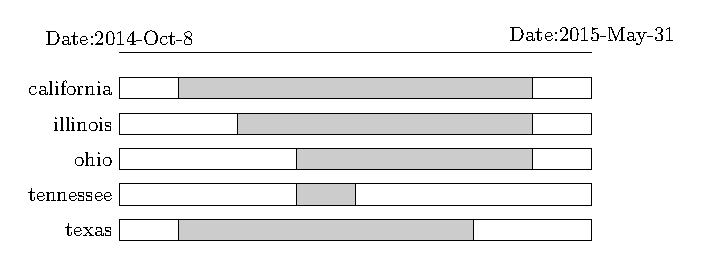
\includegraphics[width=0.45\textwidth]{tikz/seasons.pdf}
\caption{Monthly \change boundaries for top-10  active U.S. regions.}
\label{fig:seasonBoundary:US}
\end{figure}
\begin{figure}[b!]
\centering
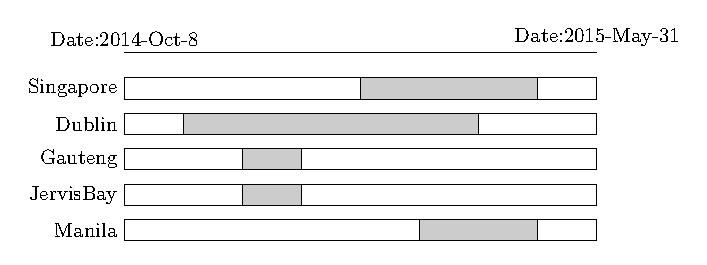
\includegraphics[width=0.45\textwidth]{tikz/seasonsNonUS.pdf}
\caption{Monthly \change boundaries for top-10 active non-U.S. regions.}
\label{fig:seasonBoundary:NonUS}
\end{figure}
\begin{table*}[t!]
\centering
\caption{$M_{full}$ transitions for California (threshold: $0.815$)}
\label{tab:fulltransitionCalifornia}
\begin{tabular}{|c|c|c|l|} \hline
Transition Type & From Topic&To Topic&Weight\\ \hline
One-Way Transitions & smoking/junkies/drugs/cigarettes & respiratory diseases&  2.70\\ 
 & depression/complaining/cursing/slangs/self-pity &  joint pains/body pains&  3.25\\
 \hline\end{tabular}
\end{table*}
\subsubsection{Topic Transitions}
Entry $m_{ij}$ in the transition parameter matrix $M$ produced by
\tmatam, shows the degree that topic $z_i$ will contribute to topic $z_j$
in the following \change. We analyze 3 kinds of transition matrices
corresponding to our setting: \textit{intra-\change}: $M_{pre}$, $M_{post}$
and  \textit{full-time-period}: $M_{full}$ .
We adapt the threshold used in \cite{DBLP:conf/kdd/WangAB12} to our settings:
\begin{equation}
Threshold  = \mu + 2\times\sigma_{non-diagonal}
\end{equation}
Here $\mu$ is the mean of the corresponding transition matrix. $\sigma_{non-diagonal}$ is the standard deviation of non-diagonal entries. We choose this threshold because 95.45\% of the values lie within two standard deviations of the mean.\footnote{\url{https://en.wikipedia.org/wiki/68-95-99.7_rule}}
We identify three kinds of 
interesting transitions based on the threshold defined in~\cite{DBLP:conf/kdd/WangAB12}:
\begin{itemize}
 \item Self transitions: Diagonal entries above threshold
 \item Symmetric Transitions: Both $m_{ij}$ and $m_{ji}$ is higher than threshold
 \item One-Way Transitions: Only one of $m_{ij}$ and $m_{ji}$ is higher than threshold
\end{itemize}
\begin{table}[t!]
\centering
\caption{$M_{full}$: California}
\label{tab:statsCalifornia}
\begin{tabular}{|c|l|} \hline
\#tweets & 55475 \\ \hline
$\mu_{full}$ & 0.015\\ \hline
$\sigma_{non-diagonal}$& 0.4\\ \hline
$\mu_{diagonal}$ & -0.002 \\ \hline
Threshold & 0.015 + $2\times0.4$ = 0.815 \\ 
 \hline\end{tabular}
\end{table}
Mean of diagonal entries is the quantification of how stable the 
transitions are and standard deviation of non-diagonal entries is 
the quantification of how much the topics fluctuate in the given 
time granularity. Let mean be denoted by $\mu$ and standard deviation 
be denoted by $\sigma$ for further discussion
\begin{table*}[t!]
\centering
\caption{$M_{full}$ (Threshold: 0.45) Transitions for Kuala Lumpur}
\label{tab:transitionKualaLumpur}
\begin{tabular}{|c|c|c|l|} \hline
Type &From Topic&To Topic&Weight\\ \hline
One-Way Transition& Heart Disease/Blood Pressure & Coughing/runny nose/watery eyes&0.85\\
 & Brain Disorder & Body pains/Weight Loss&0.599\\
 &Urinary Infection/Intestine/Tract & Stomach Pain/Blood Pressure&0.51\\
\hline\end{tabular}
\end{table*}
Table \ref{tab:statsCalifornia} summarizes the essential statistics 
of \textit{$M_{full}$} of California. As can be observed 
from 4th entry, $\mu_{diagonal}$ in Table \ref{tab:statsCalifornia} 
is almost 0 and this is intuitive because health topics transition a lot 
between \changes. Table~\ref{tab:fulltransitionCalifornia} lists 
interesting one-way health topic transitions observed in California for the full time period. Self-Transitions are hard to find
in \textit{full} time periods as topics change randomly. 
\begin{table*}[t!]
\centering
\caption{$M_{pre}$ transitions in Arizona (threshold: $0.035$)}
\label{tab:fulltransitionArizona}
\begin{tabular}{|c|c|c|l|} \hline
Transition Type & From Topic&To Topic&Weight\\ \hline
Self-Transition & Stomach Infection & Stomach Infection& 0.064\\ 
  &Headache &Headache& 0.09\\ \hline
Symmetric-Transition & Stomach Infection & Headache & 0.06\\ 
& Headache & Stomach Infection & 0.09\\
 & Stomach Infection & Pneumonia & 0.05\\ 
& Pneumonia & Stomach Infection & 0.04\\ 
 \hline\end{tabular}
\end{table*}	
\begin{table}[b!]
\centering
\caption{Transitions Stats for Kuala
Lumpur}
\label{tab:transitionStatsKualaLumpur}
\begin{tabular}{|c|l|} \hline
Statistic & Value \\ \hline
$\mu_{diagonal}$  $M_{full}$ &0.0025\\ \hline
$\mu_{diagonal}$ $M_{post}$ & 0.01 \\ \hline
$\mu_{diagonal}$  $M_{pre}$ &  0.024\\ \hline
$\sigma_{non-diagonal}$ $M_{full}$ & 0.09 \\ \hline
$\sigma_{non-diagonal}$ $M_{post}$& 0.068\\ \hline
$\sigma_{non-diagonal}$ $M_{pre}$& 0.018\\
 \hline\end{tabular}
\end{table}
\begin{table}[b!]
\centering
\caption{$M_{pre}$ (Threshold: 0.039) and $M_{post}$ (Threshold: 0.13) Transitions for Kuala Lumpur}
\label{tab:transitionKualaLumpurprepost}
\begin{tabular}{|c|c|c|l|} \hline
Type &From Topic&To Topic&Weight\\ \hline
Self Transition $M_{pre}$ & headache & headache& 0.19 \\ \hline
Self Transition $M_{post}$& body pain& body pain& 0.228\\ 
\hline\end{tabular}
\end{table}
Further, we analyze $M_{pre}$, $M_{post}$ and $M_{full}$ of Kuala\\
 Lumpur. Various statistics are summarized in Table~\ref{tab:transitionStatsKualaLumpur}.\\
 $\mu_{diagonal}$ is consistently higher for $M_{pre}$ and $M_{post}$ than $M_{full}$. $\sigma_{non-diagonal}$ is higher for
 $M_{full}$ than both \textit{intra-\change} transition matrices. These statistics go on to 
show that health topics do not drastically change and are coherent within 
the same \change and transform into one another a lot across the 
\changes. This further re-instates this fact that it is 
more sensible to model topic transition matrices within the same
\change and update them once the \change has ended. Further, 
we analyze the interesting self transitions of \textit{intra-\change}
($M_{pre}$ and $M_{post}$) and one-way transitions of $M_{full}$.
Arizona transitions are summarized in Table \ref{tab:fulltransitionArizona} and Kuala-Lumpur transitions are summarized in Tables
\ref{tab:transitionKualaLumpur} and \ref{tab:transitionKualaLumpurprepost}.

